\chapter{Lightweight Posit Processing Unit for data compression}\label{chap:posit_hw}




\section{The RISCV Instruction Set Architecture}

\lettrine{T}{he} RISC-V \cite{riscvisa} architecture is a modular, open-source and royalty-free instruction set architecture (ISA) and comprises both 32 and 64-bit architectures. The ISA is built out of small sub-ISAs. The base subsets are referred as \textit{base integer instruction sets} and identified by the letter \texttt{I}. Furthermore, a RISC-V-based architecture has additional extensions; some extension is \textit{frozen} since their encoding and behaviour has been already ratified and cannot change during the current revision of the ISA. These extensions are integer multiplication/division operations (\texttt{M}), single (\texttt{F}), double (\texttt{D}) precision floating point operations (following the IEEE 754 Float standard) and atomic instructions (\texttt{A}). In order to access the RISC-V architecture for customization of the ISA and program execution there are two ways:
\begin{itemize}
    \item The RISC-V ISA simulator (also known as Spike \cite{riscvisasim}). This simulator fully emulates the instruction set of a 64-bit RISC-V with all the extensions said above, but also with vectorization support. It provides a high-level interface to customize the instruction set, simply adding the opcodes and the behaviour of the instructions, all in C++. In order to execute compiled binaries on the Spike simulator, we must pass through the RISC-V proxy kernel, which embeds the \textit{Berkeley Boot Loader} and allows us to execute statically linked RISC-V binaries. This also comes with a customizable high-level interface where we can define the instruction opcodes. The combination of Spike and the proxy kernel allows us to execute any RISC-V binary on any other architecture for which it is compiled (e.g. x86) machine. To compile and link RISC-V binaries we used the official GCC cross compiler from the RISC-V organization repository. This allowed us to produce RISC-V binaries on an x86 host.
    \item The Ariane RISC-V FPGA core. This core is a 6-stage (2-stage speculative frontend, instruction decoding, issuing, executing and committing), single-issue, in-order CPU. It embeds a 64-bit RISC-V instruction set with \texttt{I, M, A, C} subsets. It also supports \texttt{M, S, U} privilege levels, allowing the possibility to execute any Unix-like operative system on it. The core is completely open-source and extensible using SystemVerilog.
\end{itemize}

\section{Lightweight Posit Processing Unit (PPU)}

In \cite{ppulight}, we leveraged the RISC-V custom opcode space to introduce new posit instructions inside a RISC-V processor core.
However, we decided to diverge from previous works in two different ways, one at the hardware level and the other at the software level:
\begin{itemize}
    \item At the hardware level we decided to keep our PPU$^{light}$ as light as possible, in order to adhere to RISC-V minimalism, without bringing too much additional complexity to the RISC-V core. Thus, we did not introduce new posit registers but we decided to re-use the integer ALU registers also for posit operands. This simplified extremely the integration of our PPU$^{light}$ design inside the RISC-V core. On the other hand, we only implemented conversion instructions between posits, IEEE 32-bit floats  and fixed-points, enabling quire support at a software level. Note that, once converted to a fixed-point, the sum of two posits is simply the sum of two integers: this means that we can perform true posit floating-point-like computations without involving the IEEE FP32 floating point unit at all. As a trade-off, this is, not a lossless conversion between posits and fixed-point format.
    
    Furthermore, we decided to support only $8$ and $16$ bit posits. This is because $16$-bit posits proved to be as good as IEEE floats in deep learning applications \cite{deeppositron,positnn,9066876}. Furthermore, having support for $8$-bit posits allows very fast arithmetic without having significant accuracy degradation (\cite{coco_et_al_ieeespm_2020,coco2020sensors}).
    \item At the software level we decided not to modify any element of the C compiler toolchain, making the overall software library completely portable on any modern RISC-V C compiler. We indeed make use of inline assembly instruction emission directly from C code, then wrapped in a high-level intrinsic interface. Everything is finally self-contained inside a single header file.
\end{itemize}

As a consequence of these two points, we assert that our light PPU can be used in two different ways (see Figure \ref{fig:use_cases}):
\begin{itemize}
    \item If the RISC-V processor embeds an FPU, the PPU$^{light}$ can be used as a wrapper, providing data compression by a factor up to 4, with little accuracy degradation. The cost of compression and decompression is the cost of converting a posit to a float and vice-versa.
    \item If the RISC-V processors do not embed an FPU or we want to exploit only the ALU, the PPU$^{light}$ can function as a wrapper of fixed-point representation. Indeed, once we have converted between posit and fixed-point, the basic arithmetic operations can be computed just with the ALU. Also note that, for half of the posit domain, that is the $[-1,1]$ range, the conversion between posit and the fixed point is a simple left shift of $2$ positions followed by $0$ padding on the most significant bits to reach desired fixed-point size.
\end{itemize}

Figure \ref{fig:use_cases} shows an example of the two possible approaches: in the top one, we employ the PPU$^{light}$ alongside the  FPU  and  the  ALU,  supporting  both  floating  point  and fixed  point  as  a  back-end  of  our  operation.  In  the  bottom one, we put the  PPU$^{light}$ in a scenario where only the ALU is present, thus enabling posit computation with a pure fixed-point approach. Note that in both cases, our approach is non-disruptive. This means that the existing architecture remains untouched, with just the addition of a new module. From a software-level perspective, this offers the highest transparency possible.


\begin{figure}
    \centering
    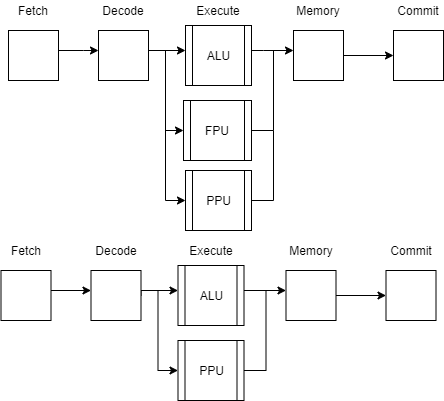
\includegraphics[width=0.5\linewidth]{img/use_cases.png}
    \caption{A visualization of the two possible use cases of the PPU$^{light}$. }
    \label{fig:use_cases}
\end{figure}


We extended the RISC-V ISA to support posit operations keeping in mind the minimalism of RISC-V. The core idea is to implement basic posit operations (addition, multiplication and others) using other wider types as backends. Therefore, we did not introduce new ad-hoc registers for posits. Instead, we aimed to reuse existing floating point and integer registers, providing conversion instructions from/to floating point (on float registers) and fixed point (on integer registers) numbers. 

Note that, unlike floating point numbers, when converting between posit and fixed point, the size of the latter depends on the posit characteristics. From now on we will refer to  a fixed point with $N$ overall bits and $N/2$ bits for the mantissa  as fx$\left<N\right>$. Then, a posit$\left<8,0\right>$ will be converted to fx$\left<16\right>$,  a posit$\left<16,0\right>$ to fx$\left<32\right>$ and a posit$\left<16,1\right>$ to fx$\left<64\right>$.

Since we employ posits with an overall size of 16 or 8 bits, we are performing a \hl{lossy} data compression by a factor of 2 or 4 if we start from an IEEE FP32 format (maintaining a similar \hl{inference} accuracy, in machine learning and neural network tasks, as demonstrated in our previous works \cite{coco_et_al_ieeespm_2020,coco2020sensors}). Moreover, even if we use a wider backend to perform computations, the data expansion is performed only within the posit processing unit. Therefore, we are transferring compressed data from memory to CPU integer/float registers. This means that just by using posits as a \hl{lossy} compressed information storage can reduce the amount of data transferred up to a factor 4.

The instruction encoding uses the suffix \texttt{'b0001011} (6 least significant bits) that is reserved for custom ISA extension.

As listed in Table \ref{tab:rvxposit}, we added the following instructions:
\begin{itemize}
    \item Floating point and posit conversions
    \begin{itemize}
        \item \texttt{FCVT.S.P8/FCVT.P8.S}: \\Float to/from posit$\left<8,0\right>$ conversion
        \item \texttt{FCVT.S.P16.0/FCVT.P16.0.S}:\\ Float to/from posit$\left<16,0\right>$ conversion
        \item \texttt{FCVT.S.P16.1/FCVT.P16.1.S}: \\Float to/from posit$\left<16,1\right>$
    \end{itemize}
    \item Fixed point and posit conversions
    \begin{itemize}
        \item \texttt{FXCVT.H.P8/FXCVT.P8.H}: \\fx$\left<16\right>$ to/from posit$\left<8,0\right>$ conversion
        \item \texttt{FXCVT.W.P16.0/FXCVT.P16.0.W}:\\ fx$\left<32\right>$ to/from posit$\left<16,0\right>$ conversion
        \item \texttt{FXCVT.L.P16.1/FXCVT.P16.1.L}: \\fx$\left<64\right>$ to/from posit$\left<16,1\right>$
    \end{itemize}   
    \item Posit to posit conversions
    \begin{itemize}
        \item \texttt{FCVT.P8.P16.0/FCVT.P16.0.P8}: \\posit$\left<8,0\right>$ to/from posit$\left<16,0\right>$ conversion
        \item \texttt{FCVT.P16.1.P16.0/FCVT.P16.0.P16.1}:\\
        posit$\left<16,1\right>$ to/from posit$\left<16,0\right>$ conversion
        \item \texttt{FCVT.P8.P16.1/FCVT.P16.1.P8}:
        \\posit$\left<16,1\right>$ to/from posit$\left<8,0\right>$ conversion
        \end{itemize}       
\end{itemize}

\begin{table*}
\caption{Instruction listing for RISC-V RVXposit extension}
\begin{small}
\begin{center}
\begin{tabular}{p{0in}p{0.4in}p{0.05in}p{0.05in}p{0.05in}p{0.05in}p{0.4in}p{0.6in}p{0.4in}p{0.6in}p{0.7in}l}
&
\multicolumn{1}{l}{\instbit{31}} &
\multicolumn{1}{r}{\instbit{27}} &
\instbit{26} &
\instbit{25} &
\multicolumn{1}{l}{\instbit{24}} &
\multicolumn{1}{r}{\instbit{20}} &
\instbitrange{19}{15} &
\instbitrange{14}{12} &
\instbitrange{11}{7} &
\instbitrange{6}{0} \\
\cline{2-11}

&
\multicolumn{4}{|c|}{1100000} &
\multicolumn{2}{c|}{00010} &
\multicolumn{1}{c|}{rs1} &
\multicolumn{1}{c|}{000} &
\multicolumn{1}{c|}{rd} &
\multicolumn{1}{c|}{0001011} & FCVT.S.P8 \\
\cline{2-11}


&
\multicolumn{4}{|c|}{1100000} &
\multicolumn{2}{c|}{00011} &
\multicolumn{1}{c|}{rs1} &
\multicolumn{1}{c|}{000} &
\multicolumn{1}{c|}{rd} &
\multicolumn{1}{c|}{0001011} & FCVT.S.P16.0 \\
\cline{2-11}


&
\multicolumn{4}{|c|}{1100000} &
\multicolumn{2}{c|}{00011} &
\multicolumn{1}{c|}{rs1} &
\multicolumn{1}{c|}{010} &
\multicolumn{1}{c|}{rd} &
\multicolumn{1}{c|}{0001011} & FCVT.S.P16.1 \\
\cline{2-11}


&
\multicolumn{4}{|c|}{1101000} &
\multicolumn{2}{c|}{00010} &
\multicolumn{1}{c|}{rs1} &
\multicolumn{1}{c|}{000} &
\multicolumn{1}{c|}{rd} &
\multicolumn{1}{c|}{0001011} & FCVT.P8.S \\
\cline{2-11}


&
\multicolumn{4}{|c|}{1101000} &
\multicolumn{2}{c|}{00011} &
\multicolumn{1}{c|}{rs1} &
\multicolumn{1}{c|}{000} &
\multicolumn{1}{c|}{rd} &
\multicolumn{1}{c|}{0001011} & FCVT.P16.0.S \\
\cline{2-11}


&
\multicolumn{4}{|c|}{1101000} &
\multicolumn{2}{c|}{00011} &
\multicolumn{1}{c|}{rs1} &
\multicolumn{1}{c|}{010} &
\multicolumn{1}{c|}{rd} &
\multicolumn{1}{c|}{0001011} & FCVT.P16.1.S \\
\cline{2-11}


&
\multicolumn{4}{|c|}{1100000} &
\multicolumn{2}{c|}{00010} &
\multicolumn{1}{c|}{rs1} &
\multicolumn{1}{c|}{001} &
\multicolumn{1}{c|}{rd} &
\multicolumn{1}{c|}{0001011} & FXCVT.H.P8 \\
\cline{2-11}


&
\multicolumn{4}{|c|}{1100000} &
\multicolumn{2}{c|}{00011} &
\multicolumn{1}{c|}{rs1} &
\multicolumn{1}{c|}{001} &
\multicolumn{1}{c|}{rd} &
\multicolumn{1}{c|}{0001011} & FXCVT.W.P16.0 \\
\cline{2-11}


&
\multicolumn{4}{|c|}{1100000} &
\multicolumn{2}{c|}{00011} &
\multicolumn{1}{c|}{rs1} &
\multicolumn{1}{c|}{011} &
\multicolumn{1}{c|}{rd} &
\multicolumn{1}{c|}{0001011} & FXCVT.L.P16.1 \\
\cline{2-11}


&
\multicolumn{4}{|c|}{1101000} &
\multicolumn{2}{c|}{00010} &
\multicolumn{1}{c|}{rs1} &
\multicolumn{1}{c|}{001} &
\multicolumn{1}{c|}{rd} &
\multicolumn{1}{c|}{0001011} & FXCVT.P8.H \\
\cline{2-11}


&
\multicolumn{4}{|c|}{1101000} &
\multicolumn{2}{c|}{00011} &
\multicolumn{1}{c|}{rs1} &
\multicolumn{1}{c|}{001} &
\multicolumn{1}{c|}{rd} &
\multicolumn{1}{c|}{0001011} & FXCVT.P16.0.W \\
\cline{2-11}


&
\multicolumn{4}{|c|}{1101000} &
\multicolumn{2}{c|}{00011} &
\multicolumn{1}{c|}{rs1} &
\multicolumn{1}{c|}{011} &
\multicolumn{1}{c|}{rd} &
\multicolumn{1}{c|}{0001011} & FXCVT.P16.1.L \\
\cline{2-11}


&
\multicolumn{4}{|c|}{1101000} &
\multicolumn{2}{c|}{00010} &
\multicolumn{1}{c|}{rs1} &
\multicolumn{1}{c|}{001} &
\multicolumn{1}{c|}{rd} &
\multicolumn{1}{c|}{0001011} & FXCVT.P8.H \\
\cline{2-11}


&
\multicolumn{4}{|c|}{1101000} &
\multicolumn{2}{c|}{00011} &
\multicolumn{1}{c|}{rs1} &
\multicolumn{1}{c|}{001} &
\multicolumn{1}{c|}{rd} &
\multicolumn{1}{c|}{0001011} & FXCVT.P16.0.W \\
\cline{2-11}


&
\multicolumn{4}{|c|}{1101000} &
\multicolumn{2}{c|}{00011} &
\multicolumn{1}{c|}{rs1} &
\multicolumn{1}{c|}{011} &
\multicolumn{1}{c|}{rd} &
\multicolumn{1}{c|}{0001011} & FXCVT.P16.1.L \\
\cline{2-11}


&
\multicolumn{4}{|c|}{1100000} &
\multicolumn{2}{c|}{00010} &
\multicolumn{1}{c|}{rs1} &
\multicolumn{1}{c|}{100} &
\multicolumn{1}{c|}{rd} &
\multicolumn{1}{c|}{0001011} & FCVT.P8.P16.0 \\
\cline{2-11}


&
\multicolumn{4}{|c|}{1100000} &
\multicolumn{2}{c|}{00011} &
\multicolumn{1}{c|}{rs1} &
\multicolumn{1}{c|}{100} &
\multicolumn{1}{c|}{rd} &
\multicolumn{1}{c|}{0001011} & FCVT.P16.0.P8 \\
\cline{2-11}


&
\multicolumn{4}{|c|}{1101000} &
\multicolumn{2}{c|}{00011} &
\multicolumn{1}{c|}{rs1} &
\multicolumn{1}{c|}{111} &
\multicolumn{1}{c|}{rd} &
\multicolumn{1}{c|}{0001011} & FCVT.P16.1.P16.0 \\
\cline{2-11}


&
\multicolumn{4}{|c|}{1101000} &
\multicolumn{2}{c|}{00010} &
\multicolumn{1}{c|}{rs1} &
\multicolumn{1}{c|}{101} &
\multicolumn{1}{c|}{rd} &
\multicolumn{1}{c|}{0001011} & FCVT.P16.1.P8 \\
\cline{2-11}


&
\multicolumn{4}{|c|}{1100000} &
\multicolumn{2}{c|}{00011} &
\multicolumn{1}{c|}{rs1} &
\multicolumn{1}{c|}{110} &
\multicolumn{1}{c|}{rd} &
\multicolumn{1}{c|}{0001011} & FCVT.P8.P16.1 \\
\cline{2-11}


&
\multicolumn{4}{|c|}{1101000} &
\multicolumn{2}{c|}{00011} &
\multicolumn{1}{c|}{rs1} &
\multicolumn{1}{c|}{101} &
\multicolumn{1}{c|}{rd} &
\multicolumn{1}{c|}{0001011} & FCVT.P16.0.P16.1 \\
\cline{2-11}


\end{tabular}
\end{center}
\end{small}
\label{tab:rvxposit}
\end{table*}


Once the instructions have been encoded we need to provide a high-level interface to use them. The idea is to implement a C intrinsic for each instruction exploiting the inline assembly \texttt{\_\_asm\_\_} operator to emit the byte code associated with the specific instruction.
This approach avoids us to implement the code generation inside the compiler. Instead, we let the compiler choose the proper registers for the intrinsic exploiting C/C++ register allocation with the keyword \texttt{register}.

Listing \ref{lst:fcvtin} shows an intrinsic example for the float to posit$\left<8,0\right>$ conversion. The many \texttt{.set} directives are used to set RISC-V register identifiers. The \texttt{.byte} directive is used to emit the four bytes that compose the instruction. Comparing the four bytes of the instruction with the encoding in Table \ref{tab:rvxposit} we can see that both \texttt{rs1} and \texttt{rd} (source and destination register) are not being explicitly set in the intrinsic. Finally, the two register allocations in the function header use the RISC-V standard register names for input and output passing.
\vspace{1em}
\begin{lstlisting}[
  caption=Intrinsic example for FCVT.S.P8,
  label=lst:fcvtin,
]
int __fcvt_f32_p8 (float a) {
 register float p1 asm (``fa0") = a;
 register int result asm (``a1");
 __asm__ volatile(
  ``"
  ``.set rfs0,8\n"
  ``.set rfs1,9\n"
  ...
  ``.set op,0xb\n"
  ``.set opf1,0x0\n"
  ``.set opf2,0x2\n"
  ``.set opf3,0x60\n"
  ``.byte  op|((r%[result]&1) <<7),
          ((r%[result]>>1)&0xF)|(opf1<<4)|((r%1&1)<<7),
          ((opf2&0xF) << 4) | ((r%1>>1)&0xF),
          ((opf2>>4)&0x1)|(opf3<<1)"
  : [result] ``=r"(result)
  :``f"(p1), ``[result]"(result));
 return result;
}
\end{lstlisting}

We instrumented the cppPosit library to be compiled with specific flags to directly use said hardware instructions instead of using software emulation. For example, without hardware support, the conversion between float and posit needs a series of bit manipulations, done in software. If we provide PPU support the same conversion results in a single call to the \texttt{FCVT.S.*/FCVT.*.S} instruction. 

This approach has three key aspects:
\begin{itemize}
    \item We implemented some core posit operations that can not be implemented as $\mathcal{L}1$ operations
    \item We discarded other slow instructions that require activation and withdrawal like in an external execution unit.
    \item We may seamlessly run in a super-scalar environment with multiple parallel execution units since we only used native integer and floating point registers.
\end{itemize}



To provide a circuit design for our PPU$^{light}$ we considered several key points to simplify the final logic design:
\begin{itemize}
    \item IEEE floating point values are encoded in a module and sign-like representation while posits are encoded using 2's complement representation. Therefore, when converting from IEEE floats we just ignore the sign and build the positive posit. Then we use the sign to apply the 2's complement to the result if negative.
    \item Given a Posit$\left<16,0\right>$ the size of the regime spans from a minimum of 2 to a maximum of 15 bits. As a result, the mantissa size spans from a minimum of 0 to a maximum of 12 bits. This means that, given a 23-bit mantissa IEEE Float, the 8 least significant bits of the float are set to 0. A similar reasoning holds for Posit$\left<8,0\right>$. 
    \item We can build the Posit$\left<X,0\right>$ regime arithmetically shifting an appropriate value by the $\log_2{X}$ least significant bits of the FP32 normalized exponent. For Posit$\left<16,0\right>$ we shift the signed integer represented by $2^{15}$ (\texttt{8000} in hexadecimal notation, as in Figure \ref{fig:fp_exp_reg_encoder}). For Posit$\left<8,0\right>$, we shift the signed integer represented by $2^{7}$. Furthermore, we always build the regime starting from the absolute value of the normalized FP32 exponent. It can be then transformed to the ``negative" regime in case of negative exponent values as in Figure \ref{fig:fp_exp_reg_encoder}. In this circuit, we take the floating point exponent on 8 bits and produce the regime bits corresponding to that exponent. To generate the regime, we arithmetically shift the signed integer represented by $2^{15}$ (\texttt{'h8000}) by the amount specified by the 4 least significant digits of the floating point exponent. The same procedure holds for both negative and positive exponents, with just a negation at the end to restore the correct sign. 
    \item Decoding the regime is particularly interesting since we need to employ a \emph{find first set} module (or \emph{find first unset}) to evaluate the regime length. The output of the \emph{find first set} module is the index $i$ of the highest set bit (discarding the sign if present). Therefore, as reported in Figure \ref{fig:fp_exp_reg_decoder}, the regime length is actually computed as $l=14-i$. In the end, the $k$-value (which is the non-normalized floating point exponent) is obtained from the regime length as $-l$ or $l+1$, depending on the regime ``sign''. In the circuit of Figure \ref{fig:fp_exp_reg_decoder}, we take the regime field and output the corresponding value of $k$. The core part is represented by the two \textit{find high} modules that help to compute the number of subsequent bit set (or unset). If we subtract this number at the maximum length of the regime (that is $14$, or \texttt{'he} in hexadecimal notation) we get the actual regime length $l$. Finally, if we follow we can retrieve $k$ from $l$.  
\end{itemize}

\begin{figure}
    \centering
    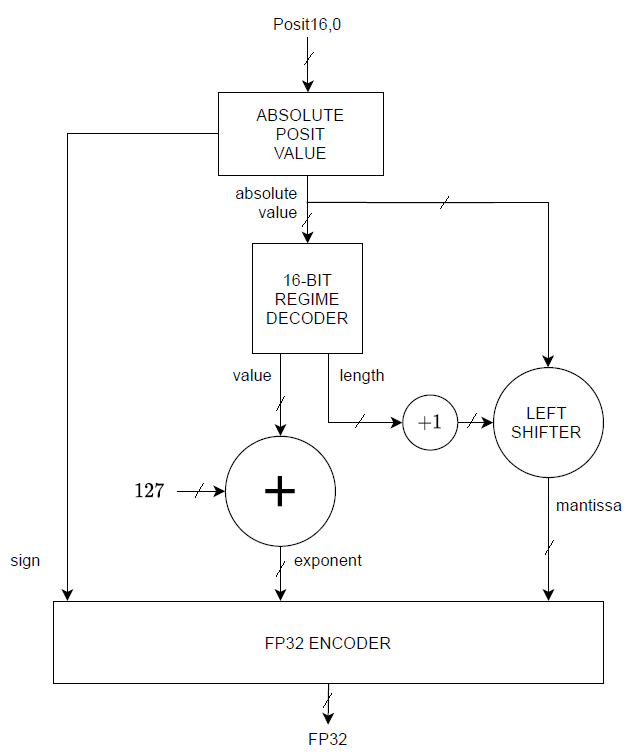
\includegraphics[width=0.5\linewidth]{img/p16_fp32.PNG}
    \caption{Logical circuit for the posit$\left<16,0\right>$ to 32-bit floating point converter.}
    \label{fig:p16_fp32_circ}
\end{figure}

\begin{figure}
    \centering
    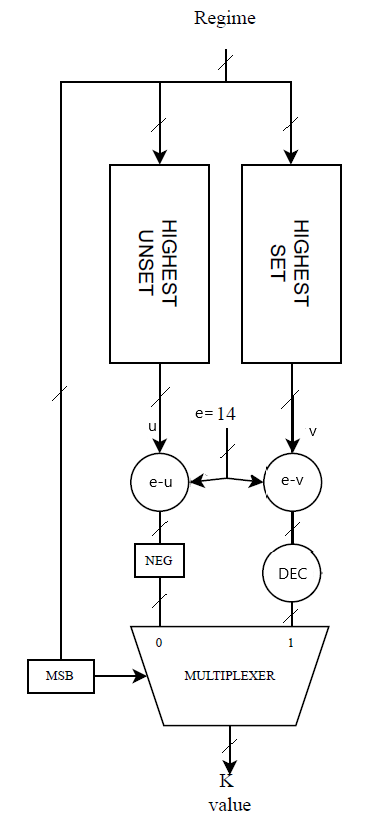
\includegraphics[width=0.56\linewidth]{img/regime_decoder.PNG}
    \caption{Logical circuit for the posit$\left<16,0\right>$ regime \textbf{decoder}}
    \label{fig:fp_exp_reg_decoder}
\end{figure}


In Figure \ref{fig:p16_fp32_circ}, we show \hl{a simplified} circuit for conversion from posit$\left<16,0\right>$ to FP32. The 16-bit regime decoder module is implemented by \hl{the simplified} circuit shown in Figure \ref{fig:fp_exp_reg_decoder}. Note how when converting to IEEE floats we firstly compute the absolute value of the posit number and then convert it to a floating point one. At the end of the circuit, we just replicate the bit sign of the posit in the bit sign of the floating point, being represented in the sign and module. 


In Figure \ref{fig:fp32_p16_circ}, we show \hl{a simplified} circuit for conversion from FP32 to posit$\left<16,0\right>$. The first multiplexer in the cascade of two multiplexers takes the exponent value as input; this input acts as a mask to detect \textit{Not A Real (NaR)} values. The 16-bit regime encoder module is implemented by \hl{the simplified} circuit shown in Figure \ref{fig:fp_exp_reg_encoder}. Note how when converting from IEEE floats we just ignore the sign and build the positive posit and then we use the sign to apply the 2's complement to the result if negative. Furthermore, we build the different posit fields considering their maximum possible length without computing any length but the regime one, making the circuit simpler.

\begin{figure}
    \centering
    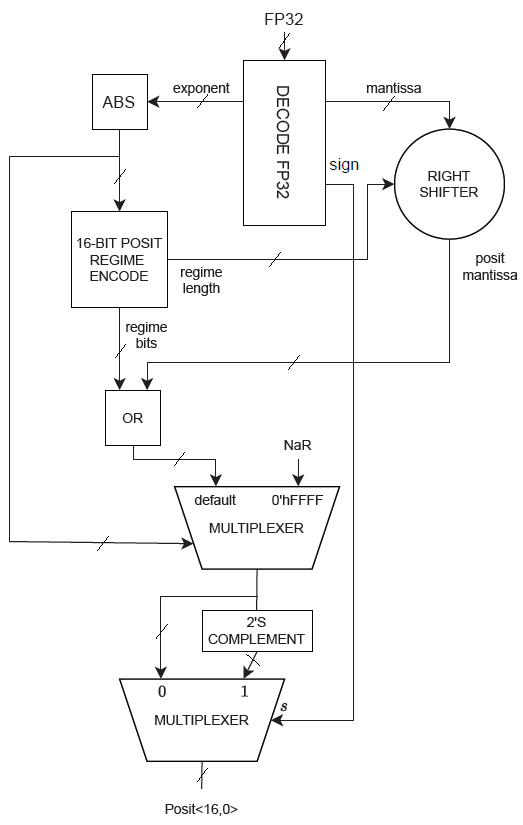
\includegraphics[width=0.5\linewidth]{img/fp32_p16.PNG}
    \caption{Logical circuit for the 32-bit floating point to posit$\left<16,0\right>$ converter. \textit{NaR} is \textit{Not A Real}.}
    \label{fig:fp32_p16_circ}
\end{figure}

\begin{figure}
    \centering
    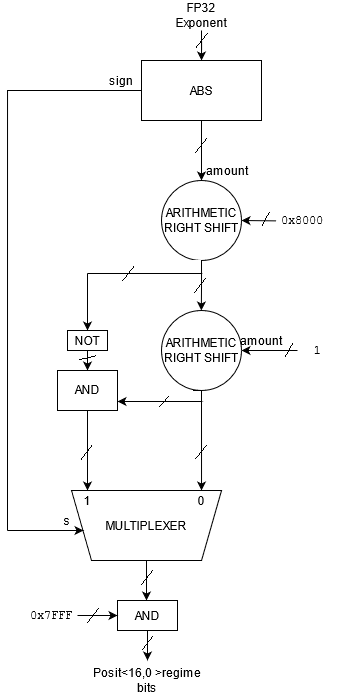
\includegraphics[width=0.5\linewidth]{img/regime_encoder.png}
    \caption{Logical circuit for the posit$\left<16,0\right>$ regime \textbf{encoder}. \textit{Amount} is the number of positions to shift the other input in the \textit{Arithmetic Right Shift} module.}
    \label{fig:fp_exp_reg_encoder}
\end{figure}



%\section{Enabling fast arithmetic operations for reals without decoding}